%% -*- Mode: LaTeX -*-
%%
%% Notes on branches in CVS.
%%

  %%
%%%%%% Preamble.
  %%

\documentclass[12pt,letterpaper]{article}

\usepackage{fancyvrb}
\usepackage{graphicx}
\usepackage{calc}
\usepackage{xspace}
\usepackage{booktabs}
%\usepackage[first,bottomafter]{draftcopy}
\usepackage[numbib]{tocbibind}

  %%
%%%%%% Customization.
  %%

% On letter paper with 10pt font the Verbatim environment has 65 columns.
% With 12pt font the environment has 62 columns.  Exceeding this will exceed
% the frame and will look ugly.  YHBW.  HAND.
\RecustomVerbatimEnvironment{Verbatim}{Verbatim}{frame=single}

\renewenvironment{description}
                 {\list{}{\labelwidth 0pt \iteminden-\leftmargin
                          \let\labelsep\hsize
                          \let\makelabel\descriptionlabel}}
                 {\endlist}
\renewcommand*\descriptionlabel[1]{\hspace\labelsep\sffamily\bfseries #1}

  %%
%%%%%% Commands.
  %%

\newcommand{\FIXME}[1]{\textsf{[FIXME: #1]}}

\newcommand{\cmd}[1]{`\texttt{#1}'}

  %%
%%%%%% Document.
  %%

\title{Notes on Branches in CVS}

\author{James A. Crippen\\
        \texttt{jcrippen@spectrumwireless.net}}

\begin{document}

\maketitle

\begin{abstract}
  Branches in CVS are presented.  The methods for creating, accessing, and
  manipulating branches are described, and the mechanism of branch and
  revision number generation is detailed.  Magic branches are described along
  with methods to handle their occasional presence.  Several methods for
  merging between different branches are presented, including methods for
  handling multiple merges between branches and the interaction of CVS
  keywords with branch merging.  Following these topics is a participatory
  walkthrough that highlights the use of each of the major concepts presented
  within the body of the work.
\end{abstract}

\tableofcontents

\listoffigures

%\listoftables



\section{Introducing Branches}

Frequently in the course of development it is necessary to concurrently
maintain two or more differing versions of files.  CVS isolates these multiple
concurrent versions in separate but related lines of development called
\emph{branches}.  When a file is changed in one branch the changes do not
appear within any other branch or in the main trunk of the file.

Occasionally the changes made in one file must be copied over to other
versions of that file.  CVS allows for the \emph{merging} of changes between
different branches of a file into the user's working copy, thus allowing the
changes to be committed to some other branch.

\subsection{Creating Branches}

A branch in CVS is represented by a special form of tag known as a
\emph{branch tag}.  Tags are managed with the \cmd{cvs tag} command; branch
tags in particular are managed through the \cmd{-b} option to this command.

Creating a branch is not difficult.  Supposing we are in a working copy
checked out of the repository, ie the current directory contains a directory
hierarchy that was checked out of a repository and includes the relevant
\cmd{CVS} directories within it.  If we wish to create a new branch of the
everything in the working copy below the current directory and assign it all
to the branch tag \cmd{rel-1-0} then we would say:

\begin{Verbatim}
# cvs tag -b rel-1-0
\end{Verbatim}

This creates a branch based on the current revisions in the working copy.
Note that this does not change the working copy.  The new branch is created in
the \emph{repository}, not in the \emph{working copy}.  The working copy still
contains exactly the same files with the exact same revisions as it did before
the branch was created.

It is also possible to create branches without referring to the working copy.
This is particulary useful when one wishes to create a branch relative to
another branch.  Creating branches relative to other branches is done with the
\cmd{cvs rtag} command.  Suppose we wish to create a branch \cmd{rel-1-0a}
that is relative to the tag \cmd{rel-1-0} of the \cmd{foo.c} file.  We say:

\begin{Verbatim}
# cvs rtag -b -r rel-1-0 rel-1-0a foo.c
\end{Verbatim}

Note again that the new branch we have created in the repository is not
represented in our working copy.



\subsection{Accessing Branches}

Accessing branches is not very different from ordinary interaction with a CVS
repository.  A branch can be checked out, updated, etc.  Checking out a branch
requires specifying the branch tag with the \cmd{-r} option.  Checking out
the \cmd{rel-1-0} branch of the \cmd{foo.c} file would entail:

\begin{Verbatim}
# cvs checkout -r rel-1-0 foo.c
\end{Verbatim}

If we already have a working copy then it can be switched to another branch.
This is done using the same \cmd{-r} option as above but for \cmd{cvs update}
instead.  Supposing we wish to change the \cmd{foo.c} file from its current
branch (perhaps the main trunk) to the \cmd{rel-1-0a} branch.  We would do:

\begin{Verbatim}
# cvs update -r rel-1-0a foo.c
\end{Verbatim}

Whether the working copy was originally on the main trunk or not, this command
will switch it to the \cmd{rel-1-0a} branch.  Unless otherwise specified, the
working copy will remain with that branch.  Thus, commits from the working
copy will add new revisions to the \cmd{rel-1-0a} branch without affecting the
main trunk or any other branches.



\section{Branches and Revisions}

Doing a \cmd{cvs status} on a file that has been branched will output the
branch tag and revision number:

\begin{Verbatim}
# cvs status -v foo.c
==============================================================
File: foo.c             Status: Up-to-date

   Working revision:    1.42    Pri Bcy 45 17:05:23 AKDT 3167
   Repository revision: 1.42    /cvs/foo/foo.c,v
   Sticky Tag:          rel-1-0a (branch 1.42.2)
   Sticky Date:         (none)
   Sticky Options:      (none)

   Existing Tags:
       rel-1-0a                     (branch: 1.42.2)
       rel-1-0                      (revision: 1.42)
\end{Verbatim}

The \cmd{Sticky Tag} field reports the current branch of the file in
question.  If we looked at another file in the same branch, say the file
\cmd{bar.c}, we might see:

\begin{Verbatim}
# cvs status -v bar.c
==============================================================
File: bar.c             Status: Up-to-date

   Working revision:    1.23    Set Cnf 19 23:42:69 AKDT 3167
   Repository revision: 1.23    /cvs/foo/bar.c,v
   Sticky Tag:          rel-1-0a (branch 1.23.2)
   Sticky Date:         (none)
   Sticky Options:      (none)

   Existing Tags:
       rel-1-0a                     (branch: 1.23.2)
       rel-1-0                      (revision: 1.23)
       rel-0-5                      (revision: 1.17)
\end{Verbatim}

Note that this file \cmd{bar.c} has revision and branch numbers that are
different from \cmd{foo.c} (eg, 1.42.2 vs 1.23.2).  The branch tag is however
the same, \cmd{rel-1-0a}.  The branch number listed in the \cmd{Existing Tags}
field reflects the point in the revision history of the file where the branch
was made.  Obviously \cmd{foo.c} has been through more revisions than
\cmd{bar.c}; when the \cmd{rel-1-0a} branch was created \cmd{foo.c} had
already been revised 42 times whereas \cmd{bar.c} had been revised only 23
times.  This demonstrates an important point regarding branch and revision
numbers versus branch tags and other tags, namely that the branch and revision
numbers are specific to one particular file.  Other files may have the same
revision and branch numbers but these numbers are only meaningful with regard
to the particular file that they are associated with.

\subsection{Revision and Branch Numbering}

The revision history of a file is usually a linearly incrementing series.  A
graph of such a revision history is shown in Figure~\ref{fig:revhist-simple}.
In this example, the file has an orderly procession of revisions starting at
1.1 and continuing to its most recent revision of 1.5.

\begin{figure}[htb]
\begin{center}

\includegraphics{revhist-simple.eps}
\end{center}
\caption{Graph of a simple, linear revision history}
\label{fig:revhist-simple}
\end{figure}

Branches provide for complex, nonlinear revision histories.  A revision
history becomes a sort of $n$-ary tree with each branch of the tree
representing a separate development path of the file.  Each branch has a
\emph{branch number} created by appending another number to the number of the
revision at the point where the branch deviated from the main trunk's
development path.

In Figure~\ref{fig:revhist-complex} the file's revision history graph is
considerably more complex.  At revision 1.2 the file was branched twice,
resulting in branches numbered 1.2.2 and 1.2.4.  The revision numbers within
each branch are incremented linearly as they are in the main trunk.  But why
is there no branch numbered 1.2.1?  This is due to the way that CVS creates
branches and how branch numbers interact with revision numbers.

\begin{figure}[htb]
\begin{center}
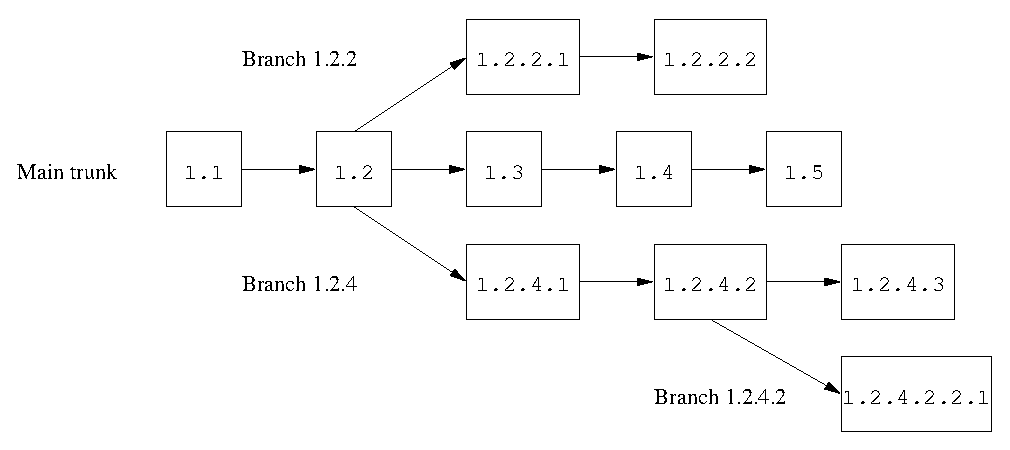
\includegraphics[width=\textwidth]{revhist-complex.eps}
\end{center}
\caption{Graph of a complex, multiply branched revision history}
\label{fig:revhist-complex}
\end{figure}

\subsubsection{Mechanics of Branch Numbering}

Branch \emph{tags} are the usual method of using and manipulating branches.
Branch numbers, which are specific to individual files, are not typically used
in day-to-day interaction with CVS.  But understanding how branch numbers are
created can help eliminate errors in specifying them and in understanding the
output of \cmd{cvs status}, amongst other reasons.

A revision number is an \emph{even} number of integers separated by periods.
A branch number is an \emph{odd} number of integers separated by periods.  1.2
is a revision number, as is 1.2.4.5.6.7.8.9.  1.2.4 is however a branch
number, as is 1.2.4.6.8.10.12.  When CVS creates a branch number it selects
the first unused \emph{even} integer, starting with 2.  Thus 1.2.1 is
\emph{not} a valid branch number, but 1.2.2 \emph{is}, being the first branch
from revision number 1.2.  Branch numbers ending in zero are used internally
to CVS and are known as \emph{magic branches} which will be discussed in a
later section.

Refer again to Figure~\ref{fig:revhist-complex}.  The file depicted in this
graph diverged twice from revision number 1.2 into branches 1.2.2 and 1.2.4.
The 1.2.2 branch was continued with two successive revisions, numbers 1.2.2.1
and 1.2.2.2. The second revision of the 1.2.4 branch, number 1.2.4.2 diverged
into branch 1.2.4.2.2.  The first revision of this branch was numbered
1.2.4.2.2.1.  Development on the 1.2.4.2 branch continued with revision
1.2.4.2 to produce the revision numbered 1.2.4.3.

The first branch of a file from a revision numbered 1.5 would be a branch
numbered 1.5.2.  The first revision of that file in the 1.5.2 branch would be
revision number 1.5.2.1.  As another example, the second branch of revision
2.23 of some file would be branch 2.23.4 (the first branch would have been
numbered 2.23.2).  A branch from the first revision of this branch (2.23.4.1)
would be branch 2.23.4.1.2 and its first revision would be 2.23.4.1.2.1.
Confused?  Be glad you're not dealing with ASN--1, which can be even
\emph{more} convoluted.

\subsubsection{Magic Branches}

Magic branches matter much less to the user than even the mechanics of branch
numbering.  Nevertheless, CVS users will occasionally encounter a branch
number that contains an extra zero in the penultimate position, ie a branch
1.2.4 becomes 1.2.0.4, and a branch 2.23.4.2.2 becomes 2.23.4.2.0.2.  The
internal reasons for why CVS does this are not particularly interesting to
anyone not trying to grok CVS's guts; suffice to say that magic branches are
created for efficiency reasons.

CVS usually does a good job of hiding magic branches, but they occasionally
creep through into positions that are user-visible.  This may occur when a
magic branch number appears in the output of \cmd{cvs log}.  This may also
occur when you cannot specify a branch tag to \cmd{cvs admin}.  In the latter
case you can use \cmd{cvs admin} to reassign a branch tag to its expected
value.  The below example would reassign the tag \cmd{rel-1-0a} to the branch
1.4.2 (with magic branch number 1.4.0.2) for the file \cmd{foo.c}.


\begin{Verbatim}
# cvs admin -Nrel-1-0a:1.4.2 foo.c
\end{Verbatim}

The above example only works if at least one revision already exists on the
branch.  Some care is necessary to avoid assigning the tag to the wrong branch
number.



\section{Merging Branches}

Typically branches are not revised unto infinity with no regard to the main
trunk or any other branches.  In many cases modifications to one branch must
be copied to other branches.  In other cases modifications to the main trunk
must be applied to some other branch.

Merging changes from one branch to the working copy can be performed using
\cmd{cvs update} with the \cmd{-j {\itshape branchname}} flag, which stands
for `join'.  With one \cmd{-j} option the changes are merged into the working
copy from where the branch was forked through the newest revision of that
branch.

\begin{figure}[htb]
\begin{center}
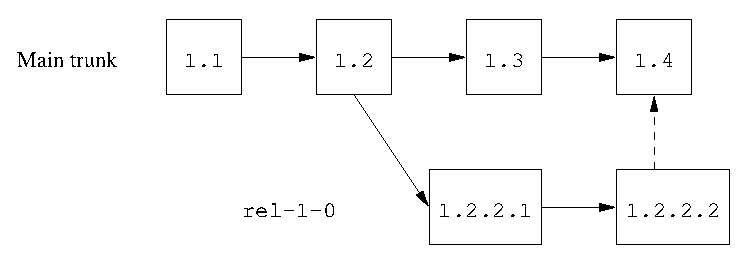
\includegraphics[width=\textwidth-1in]{revhist-bmerge.eps}
\end{center}
\caption{Merging between branches}
\label{fig:revhist-bmerge}
\end{figure}

In Figure~\ref{fig:revhist-bmerge} branch 1.2.2 is tagged \cmd{rel-1-0}.  To
merge changes from revision 1.2.2.2 to revision 1.4 (indicated by the dashed
arrow) we update our working copy (which is assumed to be up to date with the
main trunk of the repository) with the \cmd{rel-1-0} branch and then commit
these changes to the repository.  The commit of the changes is the action that
finally applies the results of the merge to the destination branch or the main
trunk.

\begin{Verbatim}
# cvs update -j rel-1-0
[...]
# cvs commit -m "Merged changes from rel-1-0."
\end{Verbatim}

Life is naturally not always as simple as the above example would indicate.
Quite often the merging of changes will result in conflicts.  It is
\emph{absolutely imperative} to resolve any conflicts that arise from the
update before committing the new version, lest the repository become muddled
with broken files full of random conflicts.

\subsection{Merging with Keywords}

When switching revisions frequently it may become confusing exactly which
revision of a file we are using at any particular moment.  Certainly \cmd{cvs 
status} can be used to answer the question, but it may be distracting to
leave the editor, open a terminal, change directories, run \cmd{cvs status},
and finally examine the output.  It is easy to forget exactly why we might
have needed to know the revision number after such a task.

A similar situation may arise when we distribute our files to other people or
places.  Since such files are no longer part of a working copy of a CVS
repository it is difficult to determine exactly which revision number a
particular file might have.  This situation is particularly frustrating
because the only simple way to determine the revision is to diff the external
version of the file against various revisions of the file from the repository
until we find a match.  Worse yet, it may not be possible to find a perfect
match because the file may have been edited since it was exported from the
repository.

CVS provides a convenient mechanism of embedding revision information in
checked out and exported files with the use of \emph{keywords}.  Keywords are
simple strings of the form ``\$$\langle$\textit{keyword-name}$\rangle$\$''
that are placed in a file to be committed.  The next time that file is checked
out from the repository CVS will expand the keyword into a string that
contains repository information about the file.  We will only consider one
keyword in this document, the ``\$Revision\$'' keyword that expands into the
file's current revision number.  Other keywords are described in detail in the
CVS documentation, and all behave in a similar manner.

If source files contain CVS keywords then spurious conflicts may arise during
merges.  To avoid this we specify the \cmd{-kk} flag on the merge command
line.  This flag substitutes the name of the keyword rather than its expanded
value, and hence ensures that the revisions being merged will not generate
spurious conflicts due to keyword substitution.

\begin{figure}[htb]
\begin{center}
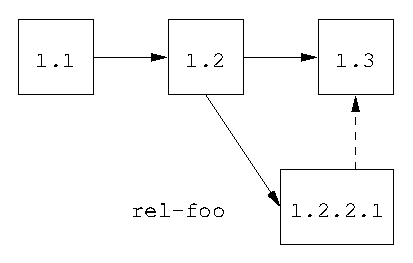
\includegraphics{revhist-kmerge.eps}
\end{center}
\caption{Merging with keywords}
\label{fig:revhist-kmerge}
\end{figure}

Suppose a file with a revision history as in Figure~\ref{fig:revhist-kmerge}.
This file happens to have the CVS ``\$Revision\$'' keyword in it.  Our working
directory is currently up to date with respect to the main trunk, in this case
with the file's revision 1.3.  Now suppose we merge the changes from the
\cmd{rel-foo} branch (branch number 1.2.2 for this file) into the trunk:

\begin{Verbatim}
# cat file-foo
$Revision: 2 $
[...]
# cvs update -j rel-foo
U file-foo
RCS file: /cvs/foo/file-foo,v
retreiving revision 1.3
retreiving revision 1.2.2.1
Merging differences between 1.3 and 1.2.2.1 into file-foo
rcsmerge: warning: conflicts during merge
# cat file-foo
<<<<<<< file-foo
$Revision: 2 $
=======
$Revision: 2 $
>>>>>>> 1.2.2.1
[...]
\end{Verbatim}

In the repository all keywords in files are stored unexpanded, ie in their
original form.  When the updates above are performed CVS follows its usual
routine of expanding any keywords found in files that it retrieves
from the repository.  In this case the keywords each expand to a different
value because their revision numbers are not the same.  When CVS tries to
merge the two files the differing strings cause a conflict.

To get around this we use the \cmd{-kk} option to disable keyword
expansion:

\begin{Verbatim}
# cat file-foo
$Revision: 2 $
[...]
# cvs update -kk -j rel-foo
U file-foo
RCS file: /cvs/foo/file-foo,v
retrieving revision 1.3
retrieving revision 1.2.2.1
Merging differences between 1.3 and 1.2.2.1 into file-foo
# cat file-foo
$Revision: 2 $
[...]
\end{Verbatim}

In this situation the \cmd{-kk} flag prevents the ``\$Revision\$'' keyword
from being expanded in either revision pulled from the repository.  Since the
text is then identical between revisions this avoids the conflict.

The \cmd{-kk} flag is not however a panacea.  It overrides \emph{any} keyword
expansion mode that CVS would normally use for a particular file, which may be
a problem if the mode was \cmd{-kb} for a binary file.  Since it is generally
a bad idea to use keywords in binary files this will usually not be a problem,
but it is important to keep in mind that with a binary file spurious conflicts
from keyword expansion may need to be dealt with by more manual means.

\subsection{Multiple Merges between Branches}

Returning to the situation in Figure~\ref{fig:revhist-bmerge}, supposing
development continued on the 1.2.2 branch following the merge between 1.2.2.2
and 1.4.  At some point we might wish to merge the new changes of the 1.2.2
branch into the main trunk, as in Figure~\ref{fig:revhist-mulbmerge}.

\begin{figure}[htb]
\begin{center}
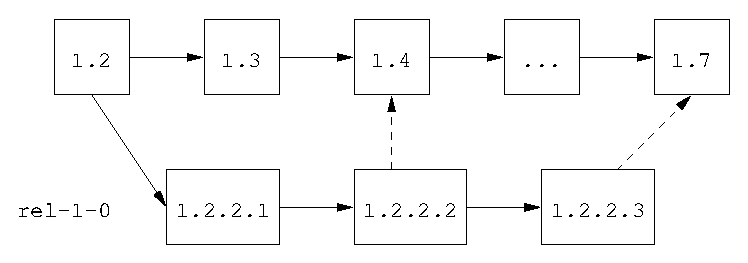
\includegraphics[width=\textwidth-1in]{revhist-mulbmerge.eps}
\end{center}
\caption{Multiple merges between branches}
\label{fig:revhist-mulbmerge}
\end{figure}

Assuming that our working copy is synchronized with revision 1.7 on the main
trunk, to merge in the new changes of the 1.2.2 branch we try using the same
technique we used to merge between branches earlier:

\begin{Verbatim}
# cvs update -j rel-1-0
[...]
# cvs commit -m "Merged more changes from rel-1-0."
\end{Verbatim}

In this case CVS na\"\i{}vely attempts to merge the changes that we had merged
in previously.  This is quite obviously not a desirable situation.  To work
around this problem it is necessary to specify that we only want to merge
changes on the branch that \emph{postdate} the last merge.  Knowing that the
last merge from branch 1.2.2 happened with revision 1.2.2.2, we want to merge
changes between that revision and number 1.2.2.3:

\begin{Verbatim}
# cvs update -j 1.2.2.2 -j rel-1-0
\end{Verbatim}

This selects only the changes from revision 1.2.2.2 to the head of the
\cmd{rel-1-0} branch, which happens to be revision 1.2.2.3.  The only drawback
with this method is that it requires specifying the 1.2.2.2 revision number
manually.  This will only work with a \emph{single file}, since different
files have different revision histories and hence different revision numbers.
Instead, a somewhat better approach might be to use the date at which the last
merge was done:

\begin{Verbatim}
# cvs update -j rel-1-0:yesterday -j rel-1-0
\end{Verbatim}

This however requires that we recall when the previous merge occurred, which
may be difficult to determine in a large project or when a long span of time
has passed.  Another solution is to tag the \cmd{rel-1-0} branch after each
merge into the trunk, then use that tag as the starting point for subsequent
merges.  Thus we tag the branch following the first merge:

\begin{Verbatim}
# cvs update -j rel-1-0
[...]
# cvs commit -m "Merged changes from rel-1-0."
# cvs tag merged_rel-1-0_to_trunk
\end{Verbatim}

Later when we wish to merge the new set of changes, we use the tag we created
previously as the starting point for determining new changes.

\begin{Verbatim}
# cvs update -j merged_rel-1-0_to_trunk -j rel-1-0
[...]
# cvs commit -m "Merged current changes from rel-1-0."
\end{Verbatim}

Unfortunately a situation will undoubtedly arise when the previous merge was
not tagged, we do not know when it happened, and we need to merge changes for
a large number of files, thus making individual merges based on file revision
numbers impractical.  In this case another solution is to simply do the update
and remove the spurious conflicts that are generated in each file by hand.
Although slow, this reduces the chances for accidentally committing bad files
into the repository, which can irritate other users of the repository to no
end.



\section{A Walkthrough}

The best way to understand exactly how branches work is to play with them.
This walkthrough will entail creating a CVS repository, checking out a working
copy of that repository, and then trivially modifying some files in order to
branch them and otherwise manipulate them.  Readers are encouraged to follow
along in their own environment.

\subsection{Initializing the Repository}

The first step necessary is to create a repository to play with.  The most
convenient place to create one is in the \$HOME directory.  So, logged in as a
non-root\footnote{The use of a non-root user alleviates some problems
  associated with a interacting with repository as root.  Particularly, the
  root user is not permitted to commit changes to a repository as this would
  require the changed files to be owned by the root user.  Such a ownership
  would open a security hole in the system that hosts the repository.} user we
create a repository in our home directory.

\begin{Verbatim}
# cd
# mkdir cvs
# export CVSROOT=$HOME/cvs
# cvs init
# ls cvs
CVSROOT
\end{Verbatim}
%$

Following this we need a place to play.  So we create a sandbox that will
contain our working copy.  Once we have a sandbox we need to create a project
and commit it to our repository.  Usually this is done by creating a
directory, using \cmd{cvs import} on the directory, and then removing the
imported directory and checking it out from the repository.  This is a bit
laborious for a simple toy, so we will cheat a little by manually creating an
empty directory in the repository, then checking it out.

\begin{Verbatim}
# mkdir sandbox
# mkdir cvs/foo
# cd sandbox
# cvs checkout foo
cvs checkout: Updating foo
\end{Verbatim}

Now we have a project that we can actually play with.  We need to generate
some files that we can revise.

\begin{Verbatim}
# cd foo
# for i in foo bar baz; do touch $i; done
# ls
CVS  bar  baz  foo
# cvs add foo bar baz
cvs add: scheduling file `foo' for addition
cvs add: scheduling file `bar' for addition
cvs add: scheduling file `baz' for addition
cvs add: use 'cvs commit' to add these files permanently
# cvs commit
[... editing commit log ...]
RCS file: /home/james/cvs/foo/bar,v
done
Checking in bar;
/home/james/cvs/foo/bar,v  <--  bar
initial revision: 1.1
done
RCS file: /home/james/cvs/foo/baz,v
done
Checking in baz;
/home/james/cvs/foo/baz,v  <--  baz
initial revision: 1.1
done
RCS file: /home/james/cvs/foo/foo,v
done
Checking in foo;
/home/james/cvs/foo/foo,v  <--  foo
initial revision: 1.1
done
\end{Verbatim}
%$

What we have done is created a few files and checked them in.  Nothing
special, but these will become our toys for testing branches on.  The three
files are now all at revision 1.1.

\subsection{Branching}

The first thing we should do is insert some content into our files and commit
them again.  This will get us beyond the first revision and will give us
something to modify for creating differences.

\begin{Verbatim}
# for i in foo bar baz; do echo "foo" >> $i; done
# cvs commit
\end{Verbatim}
%$

At this point our three files are at revision 1.2.  Now we branch them by
setting a branch tag on everything in the current directory of the working
copy.

\begin{Verbatim}
# cvs tag -b foo-branch
cvs tag: Tagging .
T bar
T baz
T foo
\end{Verbatim}

If we look at the files with \cmd{cvs status} we will find that our working
copy was unaffected by the creation of the branch.

\begin{Verbatim}
# cvs status foo
==============================================================
File: foo               Status: Up-to-date

   Working revision:    1.2     Pri Bcy 50 17:34:42 3167
   Repository revision: 1.2     /home/james/cvs/foo/foo,v
   Sticky Tag:          (none)
   Sticky Date:         (none)
   Sticky Options:      (none)
\end{Verbatim}

We will then commit more changes to the files, which will then be at revision
1.3.

\begin{Verbatim}
# for i in foo bar baz; do echo "bar" >> $i; done
# cvs commit
\end{Verbatim}
%$

\subsection{Switching Branches}

Now that we have a branch with distinct differences from the main trunk we
switch one of the files to this new branch.

\begin{Verbatim}
# cvs update -r foo-branch foo
U foo
# cvs status bar
==============================================================
File: bar               Status: Up-to-date

   Working revision:    1.3     Pri Bcy 50 17:45:20 3167
   Repository revision: 1.3     /home/james/cvs/foo/bar,v
   Sticky Tag:          (none)
   Sticky Date:         (none)
   Sticky Options:      (none)

# cvs status foo
==============================================================
File: foo               Status: Up-to-date

   Working revision:    1.2     Pri Bcy 50 17:46:21 3167
   Repository revision: 1.2     /home/james/cvs/foo/foo,v
   Sticky Tag:          foo-branch (branch: 1.2.2)
   Sticky Date:         (none)
   Sticky Options:      (none)
\end{Verbatim}

Note that the \cmd{foo} file's revision is again at 1.2, but it has a branch
number of 1.2.2.  Why isn't it revision number 1.2.2.1?  Because 1.2.2.1 would
be the \emph{first} revision of the file on branch 1.2.2, but we haven't
committed anything since the branch was created.  Thus the file is still in
its `zeroth' revision.

\begin{Verbatim}
# echo "foobar" >> foo
# cvs commit foo
[...]
# cvs status foo
==============================================================
File: foo               Status: Up-to-date

   Working revision:    1.2.2.1 Pri Bcy 50 18:01:43 3167
   Repository revision: 1.2.2.1 /home/james/cvs/foo/foo,v
   Sticky Tag:          foo-branch (branch: 1.2.2)
   Sticky Date:         (none)
   Sticky Options:      (none)
\end{Verbatim}

We have created a revision on this branch and we now find the revision number
is what we originally expected.  Revision 1.2.2.1 is not the zeroth, but the
first revision of this file on branch 1.2.2.

\begin{figure}[h]
\begin{center}
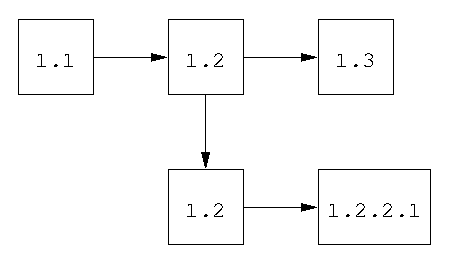
\includegraphics{walkthru-onebranch.eps}
\end{center}
\caption{Revision graph of the \cmd{foo} file}
\label{fig:walkthru-onebranch}
\end{figure}

At this point the graph of revisions on the \cmd{foo} file looks something
like the graph in Figure~\ref{fig:walkthru-onebranch}.  Unlike previous
revision graphs this graph explicitly shows the zeroth revision of the 1.2.2
branch.  Since the zeroth revision is exactly the same as the 1.2 revision
from which it was branched, it has the same revision number and the same
contents; the only difference between them is that the zeroth revision has a
branch tag, where revision 1.2 taken from the main trunk did not.  In most
situations the zeroth revision of a branch can be ignored.  It is however a
useful indicator that the file in question has not been modified since it was
branched.

\subsection{Branch Merging}

The next thing we will explore is merging between branches.  For this we will
add another revision on both branches to our files.  We'll start with the
\cmd{foo-branch}, so we need to switch all of the files in our working copy to
that branch before we do anything else.

\begin{Verbatim}
# cvs update -r foo-branch
cvs update: Updating .
U bar
U baz
# cvs status
cvs status: Examining .
==============================================================
File: bar               Status: Up-to-date

   Working revision:    1.2     Pri Bcy 50 21:01:17 3167
   Repository revision: 1.2     /home/james/cvs/foo/bar,v
   Sticky Tag:          foo-branch (branch: 1.2.2)
[...]
==============================================================
File: baz               Status: Up-to-date

   Working revision:    1.2     Pri Bcy 50 21:01:17 3167
   Repository revision: 1.2     /home/james/cvs/foo/baz,v
   Sticky Tag:          foo-branch (branch: 1.2.2)
[...]
==============================================================
File: foo               Status: Up-to-date

   Working revision:    1.2.2.1 Pri Bcy 50 21:01:17 3167
   Repository revision: 1.2.2.1 /home/james/cvs/foo/foo,v
   Sticky Tag:          foo-branch (branch: 1.2.2)
[...]
\end{Verbatim}

Note how the \cmd{bar} and \cmd{baz} files are still in their zeroth revision.
We will make some modifications to advance them to the same revision that the
\cmd{foo} file is at.  This is not necessary in real life (indeed, gratuitous
revisions are not a good idea in general), but it will make bookkeeping easier
for us in our concocted scenario because the revision tree for each file will
be the same.

\begin{Verbatim}
# echo "foobar" >> bar
# echo "foobar" >> baz
# cvs commit
\end{Verbatim}

Now we switch back to the main trunk and add another revision there.  To
switch back to the main trunk we need to clear all the sticky tags (such as
branch tags) that are set on the files in our working copy.  To do this we use
the \cmd{-A} flag to \cmd{cvs update}.  This has the effect of updating all
our files to match the latest revisions of those files on the main trunk of
the repository.

\begin{Verbatim}
# cvs update -A
cvs update: Updating .
U bar
U baz
U foo
# cvs status foo
==============================================================
File: foo               Status: Up-to-date

   Working revision:    1.3     Set Bcy 51 00:01:51 3167
   Repository revision: 1.3     /home/james/cvs/foo/foo,v
   Sticky Tag:          (none)
[...]
\end{Verbatim}

It is also possible to use the special tag \cmd{HEAD} which always specifies
the latest revision of the main trunk.  The drawback to using \cmd{cvs update 
-r HEAD} is that this still sets a sticky tag on every file, namely the
\cmd{HEAD} tag.  If we use this to get back to the latest revision for the
\cmd{foo} file, then the status of that file would be:

\begin{Verbatim}
# cvs update -r HEAD foo
U foo
# cvs status foo
==============================================================
File: foo               Status: Up-to-date

   Working revision:    1.3     Set Bcy 51 00:01:51 3167
   Repository revision: 1.3     /home/james/cvs/foo/foo,v
   Sticky Tag:          HEAD (revision: 1.3)
[...]
# cvs update -A foo
\end{Verbatim}

The final line above reverts \cmd{foo} back to its previous state which is
synchronized with the repository's main trunk.  This also removes the sticky
\cmd{HEAD} tag.  We then change the files to create a new revision, number
1.4.

\begin{Verbatim}
# for i in foo bar baz; do echo "fnord" >> $i; done
# cvs commit
\end{Verbatim}
%$

\begin{figure}[htb]
\begin{center}
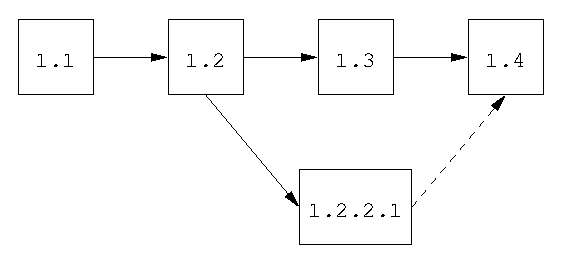
\includegraphics{walkthru-bmerge.eps}
\end{center}
\caption{Merging from \cmd{foo-branch} to the main trunk}
\label{fig:walkthru-bmerge}
\end{figure}

We are finally ready to merge between branches.  What we will do is merge
revision 1.2.2.2 into revision 1.4 as shown in
Figure~\ref{fig:walkthru-bmerge}.  To perform the merge we must first obtain
the differences between the main trunk and \cmd{foo-branch}.  We don't want to
switch branches here, we want to \emph{join} the branches.  This requires the
\cmd{-j} flag for \cmd{cvs update}.

\begin{Verbatim}
# cvs update -j foo-branch
cvs update: Updating .
RCS file: /home/james/cvs/foo/bar,v
retrieving revision 1.2
retrieving revision 1.2.2.1
Merging differences between 1.2 and 1.2.2.1 into bar
rcsmerge: warning: conflicts during merge
RCS file: /home/james/cvs/foo/baz,v
retrieving revision 1.2
retrieving revision 1.2.2.1
Merging differences between 1.2 and 1.2.2.1 into baz
rcsmerge: warning: conflicts during merge
RCS file: /home/james/cvs/foo/foo,v
retrieving revision 1.2
retrieving revision 1.2.2.1
Merging differences between 1.2 and 1.2.2.1 into foo
rcsmerge: warning: conflicts during merge
\end{Verbatim}

It appears that the files are different enough to cause conflicts.  Looking at
the \cmd{foo} file we see that CVS has helpfully pointed out the conflicting
lines in the file.

\begin{Verbatim}
# cat foo
foo
<<<<<<< foo
bar
fnord
=======
foobar
>>>>>>> 1.2.2.1
\end{Verbatim}

This isn't source code, so fixing the conflicts is trivial.  Fixing conflicts
in source code is decidedly more complicated, mostly because the computers are
much more picky than humans.  In any case, the part of the conflict marked
`foo' contains the lines from the working copy that conflicted.  The lines
below the \cmd{=======} through the conflict end marker labeled `1.2.2.1' make
up the conflicting text from the \cmd{foo-branch}, revision number 1.2.2.1.

To fix the conflict we must to edit the file by hand.  After editing we have:

\begin{Verbatim}
# cat foo
foo
bar
fnord
foobar
\end{Verbatim}

We then edit the other files in the same manner\footnote{The lazy way is to
  just copy the edited \cmd{foo} on top of \cmd{bar} and \cmd{baz} since they
  all have the same contents at this point.} and commit our new revision.

\begin{Verbatim}
# cvs commit
[...]
# cvs status foo
==============================================================
File: foo               Status: Up-to-date

   Working revision:    1.5     Set Bcy 51 00:55:25 3167
   Repository revision: 1.5     /home/james/cvs/foo/foo,v
   Sticky Tag:          (none)
[...]
\end{Verbatim}

Since the files in our working copy were checked out from the main trunk that
is where they were be committed to, and the repository now contains a new
revision, 1.5.  The updated revision tree is shown in
Figure~\ref{fig:walkthru-bmerge2}, depicting the merge of 1.4 and 1.2.2.1
together to form 1.5.

\begin{figure}[htb]
\begin{center}
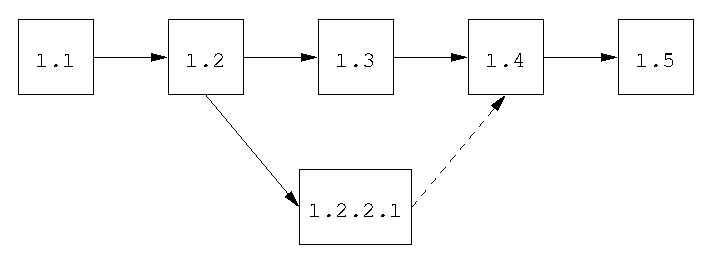
\includegraphics{walkthru-bmerge2.eps}
\end{center}
\caption{Merging 1.4 and 1.2.2.1 to form 1.5}
\label{fig:walkthru-bmerge2}
\end{figure}

\subsection{Merging with Keywords}

Because we now have two different development branches it becomes difficult to
tell at a glance which branch and revision we are working on.  We can always
tell in our working copy by using \cmd{cvs status} but this is not necessarily
an option outside of the working copy.  So it behooves us to begin using CVS
keywords.

What we will do is add a keyword to each file in both branches.  The placement
of keywords in a file is a matter of individual taste, but convention dictates
that in source code files the keyword is placed in the comment header at the
top of the file.  In human-readable documents (such as READMEs) the keyword is
typically placed at the bottom so it does not distract from the reader's
attention.  These are only conventions and not requirements, and a keyword
could just as well be placed in the middle of a file.  Such placement is
however fairly counterproductive since the keyword is supposed to be for human
use; humans are not particularly efficient at searching the contents of a file
for an arbitrary string.

\begin{Verbatim}
# for i in foo bar baz; do echo "\$Revision\$" >> $i; done
# cvs commit
\end{Verbatim}
%$

Our files are now all at revision 1.6.  If we examine one of them we should
see the expanded keyword.

\begin{Verbatim}
# cat foo
foo
bar
fnord
foobar
$Revision: 2 $
\end{Verbatim}

We then modify the \cmd{foo-branch} in the same manner.

\begin{Verbatim}
# cvs update -r foo-branch
[...]
# for i in foo bar baz; do echo "\$Revision\$" >> $i; done
# cvs commit
[...]
# cat foo
foo
foobar
$Revision: 2 $
\end{Verbatim}
%$

\begin{figure}[htb]
\begin{center}
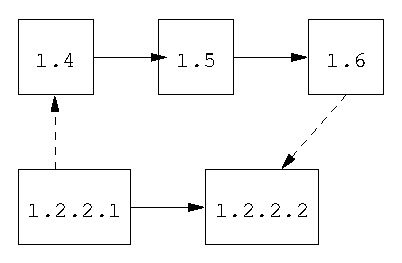
\includegraphics{walkthru-kmerge.eps}
\end{center}
\caption{Merging from the main trunk back into \cmd{foo-branch}}
\label{fig:walkthru-kmerge}
\end{figure}

Now perhaps we wish to see what would happen if we merged the main trunk into
\cmd{foo-branch}.  A graph of this merge appears in
Figure~\ref{fig:walkthru-kmerge}. We might want to do this because we're
curious whether a bug in one branch exists in the other, or maybe we're just
bored and want to have some fun (if you can call it fun).  We use the same
technique as before, joining the main trunk revision into our working copy.

\begin{Verbatim}
# cvs update -j HEAD
cvs update: Updating .
RCS file: /home/james/cvs/foo/bar,v
retrieving revision 1.2
retrieving revision 1.6
Merging differences between 1.2 and 1.6 into bar
rcsmerge: warning: conflicts during merge
\end{Verbatim}

Unsuprisingly we encountered conflicts.  Inspecting the files we find that not
only have the differences between the two branches caused conflicts, but the
``\$Revision\$'' keyword also caused conflicts due to its expansion.

\begin{Verbatim}
# cat foo
foo
<<<<<<< foo
foobar
$Revision: 2 $
=======
bar
fnord
foobar
$Revision: 2 $
>>>>>>> 1.6
\end{Verbatim}

It would be nice to exclude the keyword expansion conflicts from the other
conflicts so that we can verify what conflicts are caused by merging the two
revisions.  We revert to the last revision of the \cmd{foo-branch} and try
again, this time using the \cmd{-kk} flag to disable keyword expansion.

\begin{Verbatim}
# rm -f foo bar baz
# cvs update -kk -r foo-branch foo bar baz
cvs update: warning: foo was lost
U foo
cvs update: warning: bar was lost
U bar
cvs update: warning: baz was lost
U baz
\end{Verbatim}

CVS helpfully warns us that we removed those files and brings fresh copies
from the repository.  Since we specified \cmd{-kk} the keywords aren't
expanded.  We then merge from the main trunk again, this time without keyword
expansion.

\begin{Verbatim}
# cvs update -kk -j HEAD
cvs update: Updating .
RCS file: /home/james/cvs/foo/bar,v
retrieving revision 1.2
retrieving revision 1.6
Merging differences between 1.2 and 1.6 into bar
rcsmerge: warning: conflicts during merge
[...]
# cat foo
foo
<<<<<<< foo
foobar
$Revision: 2 $
=======
bar
fnord
foobar
$Revision: 2 $
>>>>>>> 1.6
\end{Verbatim}

The two keyword strings are still included in the file because they differ in
relation to their surrounding lines (this is because the diff program is
line-oriented).  So they still get included as conflicts, but instead of
causing the conflicts themselves they are part of one big conflict.  If we had
a complex source file that had keywords in its header comments (which rarely
change from revision to revision) then the keyword string would probably not
have appeared in a conflict at all.

\subsection{Multiple Merges}

Very commonly a branch is modified with changes that are eventually folded
back into the main trunk.  We have already merged from branches before, but
there are certain problems when we merge changes from a branch which has been
merged previously.

Suppose we wish to merge the latest changes from \cmd{foo-branch} into the
main trunk, which is currently at revision 1.6.  A graph of this merge is
given in Figure~\ref{fig:walkthru-mulbmerge}.  To merge these changes we need
changes to work with, so we will yet again append strings to our files.  After
we commit them we should have the head of \cmd{foo-branch} at revision
1.2.2.3.

\begin{Verbatim}
# cvs update -kk -r foo-branch
# for i in foo bar baz; do echo "corge grault" >> $i; done
# cvs commit
\end{Verbatim}
%$

\begin{figure}[htb]
\begin{center}
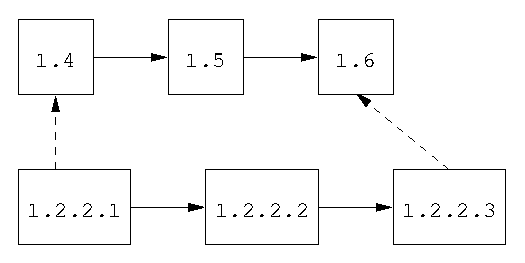
\includegraphics{walkthru-mulbmerge.eps}
\end{center}
\caption{Merging again from \cmd{foo-branch} into the main trunk}
\label{fig:walkthru-mulbmerge}
\end{figure}

If we attempt to join \cmd{foo-branch} with the main trunk without regard to
previous merges then we encounter conflicts.

\begin{Verbatim}
# rm -f foo bar baz
# cvs update -kk -A
# cvs update -kk -j foo-branch
cvs update: Updating .
RCS file: /home/james/cvs/foo/bar,v
retrieving revision 1.2
retrieving revision 1.2.2.3
Merging differences between 1.2 and 1.2.2.3 into bar
rcsmerge: warning: conflicts during merge
[...]
# cat foo
foo
<<<<<<< foo
bar
fnord
foobar
$Revision: 2 $
=======
foobar
$Revision: 2 $
corge flarp
>>>>>>> 1.2.2.3
\end{Verbatim}

To understand exactly how these conflicts arose we need to look back in the
revision history of the file.  We can use \cmd{cvs diff} to compare different
revisions of a file against each other.  The \cmd{cvs diff} command takes most
of the arguments that GNU diff accepts, as well as some specific to CVS.  Most
notable of the special CVS diff options is \cmd{-r} which selects revisions to
diff against.  This allows comparison of the working copy against a particular
revision in the repository, or of different revisions in the repository
against each other.  (The \cmd{-u} option tells diff to present a `unified
diff' which is one of the more readable formats of diff output.)

\begin{Verbatim}
# cvs diff -u -r 1.4 -r 1.2.2.1 foo
Index: foo
==============================================================
RCS file: /home/james/cvs/foo/foo,v
retrieving revision 1.4
retrieving revision 1.2.2.1
diff -u -r1.4 -r1.2.2.1
--- foo 51 Bcy 3167 00:46:46 -0000      1.4
+++ foo 51 Bcy 3167 00:45:01 -0000      1.2.2.1
@@ -1,3 +1,2 @@
 foo
-bar
-fnord
+foobar
\end{Verbatim}

The preceding diff presents the differences between revisions 1.2.2.1 and 1.4,
which were merged to become revision 1.5.  We will inspect revision 1.5 to see
how they were incorporated.

\begin{Verbatim}
# rm -f foo bar baz
# cvs update -r 1.5
[...]
# cat foo
foo
bar
fnord
foobar
\end{Verbatim}

Obviously the contents of the two files were incorporated wholesale into the
1.5 revision.  If we now look back at the results of our previous attempt at
joining \cmd{foo-branch} with the main trunk, we will see that when we tried
to join we picked up changes that had already been merged.

\begin{Verbatim}
# cvs update -kk -A
# cvs update -kk -j foo-branch
[...]
# cat foo
foo
<<<<<<< foo
bar
fnord
foobar
$Revision: 2 $
=======
foobar
$Revision: 2 $
corge flarp
>>>>>>> 1.2.2.3
\end{Verbatim}

The line containing the string ``foobar'' is the culprit.  That particular
string was absorbed into the main trunk when we merged revision 1.2.2.1 and
1.4 to produce 1.5.  What we need to do is specify that we only want to join
changes in the \cmd{foo-branch} from the 1.2.2.2 revision onwards, that is
\emph{postdating} the previous merge.

\begin{Verbatim}
# rm -f foo bar baz
# cvs update -kk -A
[...]
# cvs update -kk -j 1.2.2.2 -j foo-branch
cvs update: Updating .
RCS file: /home/james/cvs/foo/bar,v
retrieving revision 1.2.2.2
retrieving revision 1.2.2.3
Merging differences between 1.2.2.2 and 1.2.2.3 into bar
[...]
\end{Verbatim}

And so we see no conflicts.  The only thing remaining to be done is the
commission of this new revision to the repository.  After committal our
revision tree will look something like Figure~\ref{fig:walkthru-mulbmerge2}.

\begin{figure}[htb]
\begin{center}
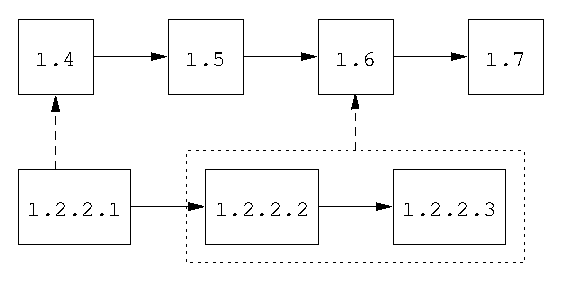
\includegraphics{walkthru-mulbmerge2.eps}
\end{center}
\caption{Merging \cmd{foo-branch} from 1.2.2.2 onwards into the main trunk}
\label{fig:walkthru-mulbmerge2}
\end{figure}



\section{Conclusion}

At first encounter, CVS branches seem confusing.  They become perhaps more
confusing when we realize that they are implemented using tags.  But branches
in CVS are not as confusing as most people believe.  The interactions with
branches are much more complicated than the simple `checkout, edit, commit,
update' process, but in complex software development projects they become
invaluable for maintaining state that would otherwise be available only on
paper or in a person's head.  Branches are also essential for developing
software in more than one direction at the same time, for instance a release
version and an internal development version.  Thus a person using CVS who does
not learn to appreciate and utilize the branching features is at a
disadvantage to those who do understand branching and can use its
functionality effectively.


\end{document}

%% Local Variables:
%% fill-column: 78
%% mode: auto-fill
%% compile-command: "make cvs-branches.dvi"
%% End:

